\documentclass[article]{jss}
\usepackage[utf8]{inputenc}

\providecommand{\tightlist}{%
  \setlength{\itemsep}{0pt}\setlength{\parskip}{0pt}}

\author{
John Ehrlinger\\Microsoft, Machine Learning COGS
}
\title{\pkg{ggRandomForests}: Regression \pkg{randomForestSRC}}
\Keywords{random forest, regression, VIMP, minimal depth, \proglang{R}, \pkg{randomForest}, \pkg{randomForestSRC}, \pkg{ggRandomForests}}

\Abstract{
Random Forests \citep{Breiman:2001} (RF) are a non-parametric
statistical method requiring no distributional assumptions on covariate
relation to the response. RF are a robust, nonlinear technique that
optimizes predictive accuracy by fitting an ensemble of trees to
stabilize model estimates. The \pkg{randomForestSRC} package
\citep{Ishwaran:RFSRC:2014} is a unified treatment of Breiman's random
forests for survival, regression and classification problems.

Predictive accuracy make RF an attractive alternative to parametric
models, though complexity and interpretability of the forest hinder
wider application of the method. We introduce the \pkg{ggRandomForests}
package, tools for visually understand random forest models grown in
\texttt{R} \citep{rcore} with the \pkg{randomForestSRC} package. The
\pkg{ggRandomForests} package is structured to extract intermediate data
objects from \pkg{randomForestSRC} objects and generates figures using
the \pkg{ggplot2} \citep{Wickham:2009} graphics package

This document is structured as a tutorial for building random forests
for regression with the \pkg{randomForestSRC} package and using the
\pkg{ggRandomForests} package for investigating how the forest is
constructed. We investigate the Boston Housing data
\citep[\citet{Belsley:1980}]{Harrison:1978}. We demonstrate random
forest variable selection using Variable Importance (VIMP)
\citep{Breiman:2001} and Minimal Depth \citep{Ishwaran:2010}, a property
derived from the construction of each tree within the forest. We will
also demonstrate the use of variable dependence plots
\citep{Friedman:2000} to aid interpretation RF results. We then examine
variable interactions between covariates using a minimal depth
interactions, and conditional variable dependence plots. The goal of the
exercise is to demonstrate the strength of using Random Forest methods
for both prediction and information retrieval in regression settings.
}

\Plainauthor{John Ehrlinger}
\Plaintitle{ggRandomForests: Regression randomForestSRC}
\Shorttitle{\pkg{ggRandomForests}: Regression \pkg{randomForestSRC}}
\Plainkeywords{random forest, regression, VIMP, minimal depth, R, randomForest, randomForestSRC, ggRandomForests}

%% publication information
%% \Volume{50}
%% \Issue{9}
%% \Month{June}
%% \Year{2012}
\Submitdate{}
%% \Acceptdate{2012-06-04}

\Address{
    John Ehrlinger\\
  Microsoft, Machine Learning COGS\\
  One Memorial Drive Cambridge, MA 02142\\
  E-mail: \href{mailto:john.ehrlinger@gmail.com}{\nolinkurl{john.ehrlinger@gmail.com}}\\
  URL: \url{https://github.com/ehrlinger/ggRandomForests}\\~\\
  }

\usepackage{natbib} \usepackage{booktabs} \usepackage{longtable}
\usepackage{amsmath} \usepackage{amsthm, amssymb}

\begin{document}

\section{About this document}\label{about-this-document}

This document is a package vignette for the \pkg{ggRandomForests}
package for ``Visually Exploring Random Forests''
(\url{http://CRAN.R-project.org/package=ggRandomForests}). The
\pkg{ggRandomForests} package is designed for use with the
\pkg{randomForestSRC} package
(\url{http://CRAN.R-project.org/package=randomForestSRC})
\citep{Ishwaran:RFSRC:2014} for growing random forests for survival
(time to event response), regression (continuous response) and
classification (categorical response) settings and uses the
\pkg{ggplot2} package (\url{http://CRAN.R-project.org/package=ggplot2})
\citep{Wickham:2009} for plotting diagnostic and variable association
results. \pkg{ggRandomForests} is structured to extract data objects
from \pkg{randomForestSRC} objects and provides functions for printing
and plotting these objects.

The vignette is a tutorial for using the \pkg{ggRandomForests} package
with the \pkg{randomForestSRC} package for building and post-processing
random forests for regression settings. In this tutorial, we explore a
random forest for regression model constructed for the Boston housing
data set \citep[\citet{Belsley:1980}]{Harrison:1978}, available in the
\texttt{MASS} package \citep{mass:2002}. We grow a random forest and
demonstrate how \pkg{ggRandomForests} can be used when determining how
the response depends on predictive variables within the model. The
tutorial demonstrates the design and usage of many of
\pkg{ggRandomForests} functions and features and also how to modify and
customize the resulting \texttt{ggplot} graphic objects along the way.

The vignette is written in \LaTeX using the \texttt{knitr} package
(\url{http://CRAN.R-project.org/package=knitr}{]}\citep[\citet{Xie:2014},\citet{Xie:2013}]{Xie:2015},
which facilitates weaving \texttt{R} \citep{rcore} code, results and
figures into document text. Throughout this document, \texttt{R} code
will be displayed in \emph{code blocks} as shown below. This code block
loads the \texttt{R} packages required to run the source code listed in
code blocks throughout the remainder of this document.

\begin{CodeChunk}

\begin{CodeInput}
R> ################## Load packages ##################
R> library("ggplot2")         # Graphics engine
R> library("RColorBrewer")    # Nice color palettes
R> library("plot3D")          # for 3d surfaces. 
R> library("dplyr")           # Better data manipulations
R> library("tidyr")           # gather variables into long format
R> library("parallel")        # mclapply for multicore processing
R> 
R> # Analysis packages.
R> library("randomForestSRC") # random forests for survival, regression and 
R>                            # classification
R> library("ggRandomForests") # ggplot2 random forest figures (This!)
R> 
R> ################ Default Settings ##################
R> theme_set(theme_bw())     # A ggplot2 theme with white background
R> 
R> ## Set open circle for censored, and x for events 
R> event.marks <- c(1, 4)
R> event.labels <- c(FALSE, TRUE)
R> 
R> ## We want red for death events, so reorder this set.
R> strCol <- brewer.pal(3, "Set1")[c(2,1,3)]
\end{CodeInput}
\end{CodeChunk}

This vignette is available within the \pkg{ggRandomForests} package on
the Comprehensive R Archive Network (CRAN)
(\{)\url{http://cran.r-project.org}) \citep{rcore}. Once the package has
been installed, the vignette can be viewed directly from within
\texttt{R} with the following command:

\begin{CodeChunk}

\begin{CodeInput}
R> vignette("randomForestSRC-Regression", package = "ggRFVignette")
\end{CodeInput}
\end{CodeChunk}

A development version of the \pkg{ggRandomForests} package is also
available on GitHub (\url{https://github.com}). We invite comments,
feature requests and bug reports for this package at
(\url{https://github.com/ehrlinger/ggRandomForests}).

\section{Introduction}\label{introduction}

Random Forests \citep{Breiman:2001} (RF) are a fully non-parametric
statistical method which requires no distributional or functional
assumptions on covariate relation to the response. RF is a robust,
nonlinear technique that optimizes predictive accuracy by fitting an
ensemble of trees to stabilize model estimates. Random Survival Forests
(RSF) \citep[\citet{Ishwaran:2008}]{Ishwaran:2007a} are an extension of
Breiman's RF techniques to survival settings, allowing efficient
non-parametric analysis of time to event data. The \pkg{randomForestSRC}
package \citep{Ishwaran:RFSRC:2014} is a unified treatment of Breiman's
random forests for survival (time to event response), regression
(continuous response) and classification (categorical response)
problems.

Predictive accuracy make RF an attractive alternative to parametric
models, though complexity and interpretability of the forest hinder
wider application of the method. We introduce the \pkg{ggRandomForests}
package for visually exploring random forest models. The
\pkg{ggRandomForests} package is structured to extract intermediate data
objects from \pkg{randomForestSRC} objects and generate figures using
the \pkg{ggplot2} graphics package \citep{Wickham:2009}.

Many of the figures created by the \pkg{ggRandomForests} package are
also available directly from within the \pkg{randomForestSRC} package.
However \pkg{ggRandomForests} offers the following advantages:

\begin{itemize}
\item
  Separation of data and figures: \pkg{ggRandomForests} contains
  functions that operate on either the \texttt{randomForestSRC::rfsrc}
  forest object directly, or on the output from \pkg{randomForestSRC}
  post processing functions (i.e. \texttt{plot.variable},
  \texttt{var.select}, \texttt{find.interaction}) to generate
  intermediate \pkg{ggRandomForests} data objects. Functions are provide
  to further process these objects and plot results using the
  \pkg{ggplot2} graphics package. Alternatively, users can use these
  data objects for their own custom plotting or analysis operations.
\item
  Each data object/figure is a single, self contained object. This
  allows simple modification and manipulation of the data or
  \pkg{ggplot2} objects to meet users specific needs and requirements.
\item
  The use of \pkg{ggplot2} for plotting. We chose to use the
  \pkg{ggplot2} package for our figures to allow users flexibility in
  modifying the figures to their liking. Each plot function returns
  either a single \texttt{ggplot} object, or a \texttt{list} of
  \texttt{ggplot} objects, allowing users to use additional
  \pkg{ggplot2} functions or themes to modify and customize the figures
  to their liking.
\end{itemize}

This document is formatted as a tutorial for using the
\pkg{randomForestSRC} package for building and post-processing random
forest models with the \pkg{ggRandomForests} package for investigating
how the forest is constructed. In this tutorial, we use the Boston
Housing Data (\autoref{data-boston-housing-values}), available in the
\texttt{MASS} package \citep{mass:2002}, to build a random forest for
regression (\autoref{random-forest---regression}) and demonstrate the
tools in the \pkg{ggRandomForests} package for examining the forest
construction.

Random forests are not parsimonious, but use all variables available in
the construction of a response predictor. We demonstrate a random forest
variable selection (\autoref{variable-selection}) process using the
Variable Importance (\autoref{variable-importance}) measure (VIMP)
\citep{Breiman:2001} as well as Minimal Depth (\autoref{minimal-depth})
\citep{Ishwaran:2010}, a property derived from the construction of each
tree within the forest, to assess the impact of variables on forest
prediction.

Once we have an idea of which variables we are want to investigate
further, we will use variable dependence plots \citep{Friedman:2000} to
understand how a variable is related to the response. Marginal variable
dependence (\autoref{variable-dependence}) plots give us an idea of the
overall trend of a variable/response relation, while partial dependence
(\autoref{partial-dependence}) plots show us a risk adjusted relation.
These figures may show strongly non-linear variable/response relations
that are not easily obtained through a parametric approach. We are also
interested in examining variable interactions
(\autoref{variable-importance}) within the forest model. Using a minimal
depth approach, we can quantify how closely variables are related within
the forest, and generate marginal dependence coplots(\autoref{coplots})
and partial dependence coplots (\autoref{partial-dependence-coplots})
(risk adjusted) conditioning plots (coplots)
\citep[\citet{cleveland:1993}]{chambers:1992} to examine these
interactions graphically.

\section{Data: Boston Housing Values}\label{data-boston-housing-values}

The Boston Housing data is a standard benchmark data set for regression
models. It contains data for 506 census tracts of Boston from the 1970
census \citep[\citet{Belsley:1980}]{Harrison:1978}. The data is
available in multiple \texttt{R} packages, but to keep the installation
dependencies for the \pkg{ggRandomForests} package down, we will use the
data contained in the \texttt{MASS} package
(\url{http://CRAN.R-project.org/package=MASS}) \citep{mass:2002},
available with the base install of \texttt{R}. The following code block
loads the data into the environment. We include a table of the Boston
data set variable names, types and descriptions for reference when we
interpret the model results.

\begin{CodeChunk}

\begin{CodeInput}
R> # Load the Boston Housing data
R> data(Boston, package="MASS")
R> 
R> # Set modes correctly. For binary variables: transform to logical
R> Boston$chas <- as.logical(Boston$chas)
\end{CodeInput}
\end{CodeChunk}

\begin{longtable}[]{@{}lll@{}}
\caption{\texttt{Boston} housing data dictionary.}\tabularnewline
\toprule
Variable & Description & type\tabularnewline
\midrule
\endfirsthead
\toprule
Variable & Description & type\tabularnewline
\midrule
\endhead
crim & Crime rate by town. & numeric\tabularnewline
zn & Proportion of residential land zoned for lots over 25,000 sq.ft. &
numeric\tabularnewline
indus & Proportion of non-retail business acres per town. &
numeric\tabularnewline
chas & Charles River (tract bounds river). & logical\tabularnewline
nox & Nitrogen oxides concentration (10 ppm). & numeric\tabularnewline
rm & Number of rooms per dwelling. & numeric\tabularnewline
age & Proportion of units built prior to 1940. & numeric\tabularnewline
dis & Distances to Boston employment center. & numeric\tabularnewline
rad & Accessibility to highways. & integer\tabularnewline
tax & Property tax rate per \$10,000. & numeric\tabularnewline
ptratio & Pupil teacher ratio by town. & numeric\tabularnewline
black & Proportion of blacks by town. & numeric\tabularnewline
lstat & Lower status of the population (percent). &
numeric\tabularnewline
medv & Median value of homes (\$1000s). & numeric\tabularnewline
\bottomrule
\end{longtable}

The main objective of the Boston Housing data is to investigate
variables associated with predicting the median value of homes
(continuous \texttt{medv} response) within 506 suburban areas of Boston.

\subsection{Exploratory Data Analysis}\label{exploratory-data-analysis}

It is good practice to view your data before beginning an analysis,
what\citep{Tukey:1977} refers to as Exploratory Data Analysis (EDA). To
facilitate this, we use \pkg{ggplot2} figures with the
\texttt{ggplot2::facet\_wrap} command to create two sets of panel plots,
one for categorical variables with boxplots at each level, and one of
scatter plots for continuous variables. Each variable is plotted along a
selected continuous variable on the X-axis. These figures help to find
outliers, missing values and other data anomalies in each variable
before getting deep into the analysis. We have also created a separate
\texttt{shiny} app (\url{http://shiny.rstudio.com}) \citep{shiny:2015},
available at (\url{https://ehrlinger.shinyapps.io/xportEDA}), for
creating similar figures with an arbitrary data set, to make the EDA
process easier for users.

The Boston housing data consists almost entirely of continuous
variables, with the exception of the ``Charles river'' logical variable.
A simple EDA visualization to use for this data is a single panel plot
of the continuous variables, with observation points colored by the
logical variable. Missing values in our continuous variable plots are
indicated by the rug marks along the x-axis, of which there are none in
this data. We used the Boston housing response variable, the median
value of homes (\texttt{medv}), for X variable.

\begin{CodeChunk}

\begin{CodeInput}
R> # Use tidyr::gather to transform the data into long format.
R> dta <- gather(Boston, variable, value, -medv, -chas)
R> 
R> # plot panels for each covariate colored by the logical chas variable.
R> ggplot(dta)+
R+   geom_point(alpha=0.4, aes(x=medv, y=value, color=chas))+
R+   geom_smooth(aes(x=medv, y=value), se=FALSE)+ 
R+   labs(y="", x=st.labs["medv"]) +
R+   scale_color_brewer(palette="Set2")+
R+   facet_wrap(~variable, scales="free_y", ncol=3)
\end{CodeInput}
\begin{figure}

{\centering 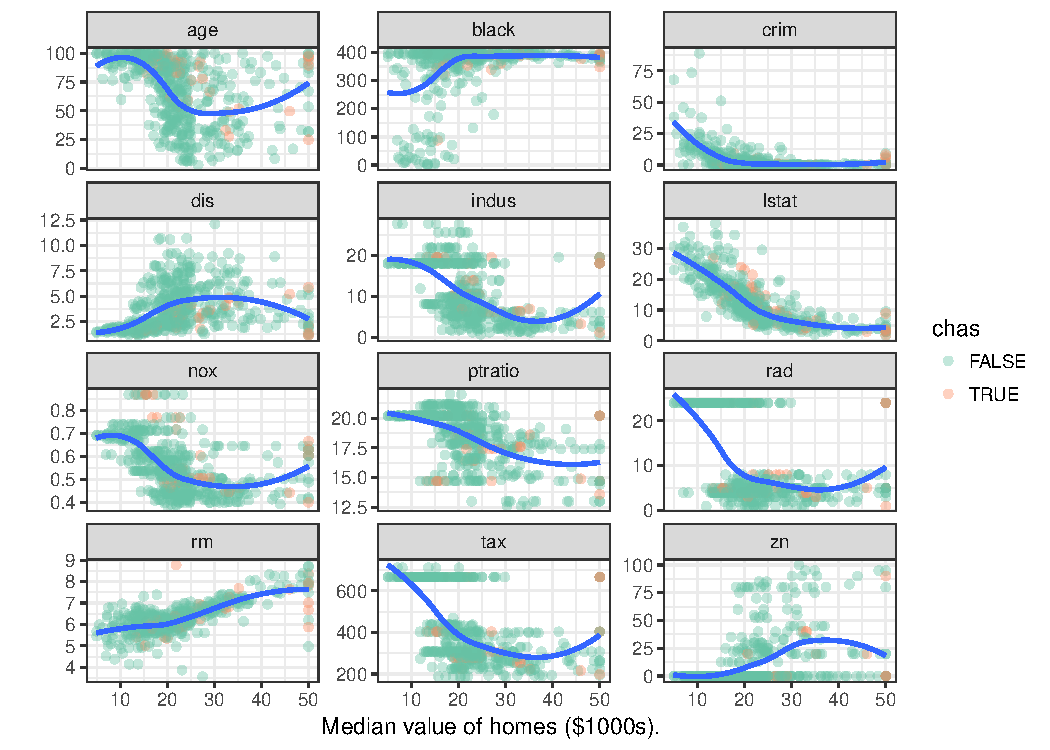
\includegraphics{Regression-rfsrc_files/figure-latex/eda-1} 

}

\caption[EDA variable plots]{EDA variable plots. Points indicate variable value against the median home value variable. Points are colored according to the chas variable.}\label{fig:eda}
\end{figure}
\end{CodeChunk}

This figure is loosely related to a pairs scatter plot
\citep{Becker:1988}, but in this case we only examine the relation
between the response variable against the remainder. Plotting the data
against the response also gives us a ``sanity check'' when viewing our
model results. It's pretty obvious from this figure that we should find
a strong relation between median home values and the \texttt{lstat} and
\texttt{rm} variables.

\section{Random Forest - Regression}\label{random-forest---regression}

A Random Forest is grown by \emph{bagging} \citep{Breiman:1996} a
collection of \emph{classification and regression trees} (CART)
\citep{cart:1984}. The method uses a set of \(B\) bootstrap
\citep{bootstrap:1994} samples, growing an independent tree model on
each sub-sample of the population. Each tree is grown by recursively
partitioning the population based on optimization of a \emph{split rule}
over the \(p\)-dimensional covariate space. At each split, a subset of
\(m \le p\) candidate variables are tested for the split rule
optimization, dividing each node into two daughter nodes. Each daughter
node is then split again until the process reaches the \emph{stopping
criteria} of either \emph{node purity} or \emph{node member size}, which
defines the set of \emph{terminal (unsplit) nodes} for the tree. In
regression trees, the split rule is based on minimizing the mean squared
error, whereas in classification problems, the Gini index is used
\citep{Friedman:2000}.

Random Forests sort each training set observation into one unique
terminal node per tree. Tree estimates for each observation are
constructed at each terminal node, among the terminal node members. The
Random Forest estimate for each observation is then calculated by
aggregating, averaging (regression) or votes (classification), the
terminal node results across the collection of \(B\) trees.

For this tutorial, we grow the random forest for regression using the
\texttt{rfsrc} command to predict the median home value (\texttt{medv}
variable) using the remaining 13 independent predictor variables. For
this example we will use the default set of \(B=1000\) trees
(\texttt{ntree} argument), \(m=5\) candidate variables (\texttt{mtry})
for each split with a stopping criteria of at most \texttt{nodesize=5}
observations within each terminal node.

Because growing random forests are computationally expensive, and the
\pkg{ggRandomForests} package is targeted at the visualization of random
forest objects, we will use cached copies of the \pkg{randomForestSRC}
objects throughout this document. We include the cached objects as data
sets in the \pkg{ggRandomForests} package. The actual \texttt{rfsrc}
calls are included in comments within code blocks.

\begin{CodeChunk}

\begin{CodeInput}
R> # Load the data, from the call:
R> rfsrc_Boston <- rfsrc(medv~., data=Boston, 
R+                       importance = TRUE, tree.err = TRUE)
R> 
R> # print the forest summary
R> rfsrc_Boston
\end{CodeInput}

\begin{CodeOutput}
                         Sample size: 506
                     Number of trees: 1000
          Minimum terminal node size: 5
       Average no. of terminal nodes: 104.22
No. of variables tried at each split: 5
              Total no. of variables: 13
                            Analysis: RF-R
                              Family: regr
                      Splitting rule: mse
                % variance explained: 87.23
                          Error rate: 10.8
\end{CodeOutput}
\end{CodeChunk}

The \texttt{randomForestSRC::print.rfsrc} summary details the parameters
used for the \texttt{rfsrc} call described above, and returns variance
and generalization error estimate from the forest training set. The
forest is built from 506 observations and 13 independent variables. It
was constructed for the continuous \texttt{medv} variable using
\texttt{ntree=1000} regression (\texttt{regr}) trees, randomly selecting
5 candidate variables at each node split, and terminating nodes with no
fewer than 5 observations.

\subsection{Generalization error
estimates}\label{generalization-error-estimates}

One advantage of Random Forests is a built in generalization error
estimate. Each bootstrap sample selects approximately 63.2\% of the
population on average. The remaining 36.8\% of observations, the
Out-of-Bag (OOB) \citep{BreimanOOB:1996e} sample, can be used as a hold
out test set for each of the trees in the forest. An OOB prediction
error estimate can be calculated for each observation by predicting the
response over the set of trees which were NOT trained with that
particular observation. The Out-of-Bag prediction error estimates have
been shown to be nearly identical to n--fold cross validation estimates
\citep{StatisticalLearning:2009}. This feature of Random Forests allows
us to obtain both model fit and validation in one pass of the algorithm.

The \texttt{gg\_error} function operates on the
\texttt{randomForestSRC::rfsrc} object to extract the error estimates as
the forest is grown. The code block demonstrates part the
\pkg{ggRandomForests} design philosophy, to create separate data objects
and provide functions to operate on the data objects. The following code
block first creates a \texttt{gg\_error} object, then uses the
\texttt{plot.gg\_error} function to create a \texttt{ggplot} object for
display.

\begin{CodeChunk}

\begin{CodeInput}
R> # Plot the OOB errors against the growth of the forest.
R> gg_e <- gg_error(rfsrc_Boston)
R> plot(gg_e)
\end{CodeInput}
\begin{figure}

{\centering 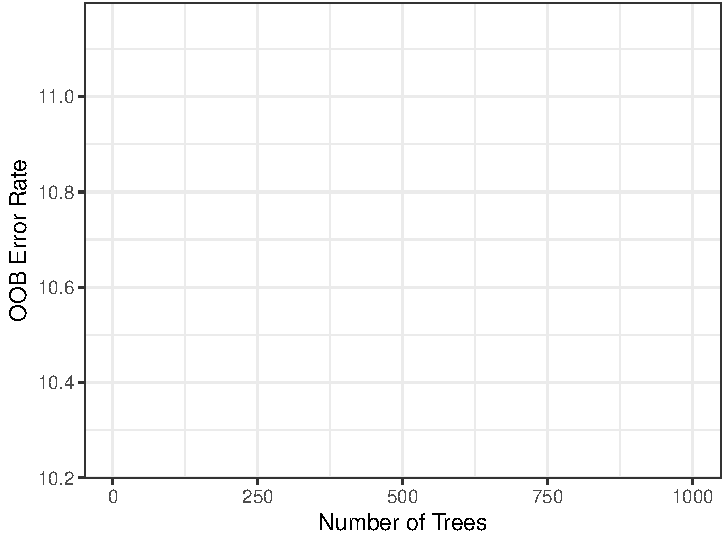
\includegraphics{Regression-rfsrc_files/figure-latex/error-1} 

}

\caption[Random forest generalization error]{Random forest generalization error. OOB error convergence along the number of trees in the forest.}\label{fig:error}
\end{figure}
\end{CodeChunk}

This figure demonstrates that it does not take a large number of trees
to stabilize the forest prediction error estimate. However, to ensure
that each variable has enough of a chance to be included in the forest
prediction process, we do want to create a rather large random forest of
trees.

\subsection{Random Forest Prediction}\label{random-forest-prediction}

The \texttt{gg\_rfsrc} function extracts the OOB prediction estimates
from the random forest. This code block executes the the data extraction
and plotting in one line, since we are not interested in holding the
prediction estimates for later reuse. Also note that we add in the
additional \pkg{ggplot2} command (\texttt{coord\_cartesian}) to modify
the plot object. Each of the \pkg{ggRandomForests} plot commands return
\texttt{ggplot} objects, which we can also store for modification or
reuse later in the analysis.

\begin{CodeChunk}

\begin{CodeInput}
R> # Plot predicted median home values.
R> plot(gg_rfsrc(rfsrc_Boston), alpha=.5)+
R+   coord_cartesian(ylim=c(5,49))
\end{CodeInput}
\begin{figure}

{\centering 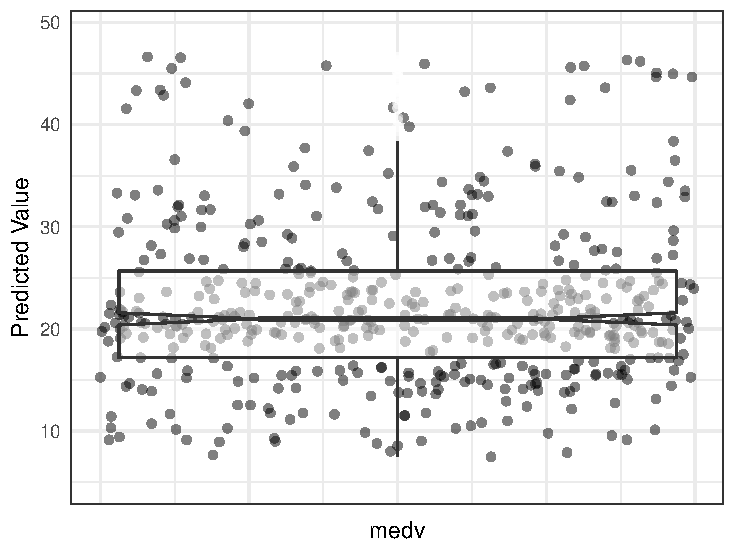
\includegraphics{Regression-rfsrc_files/figure-latex/rfsrc-1} 

}

\caption[OOB predicted median home values]{OOB predicted median home values. Points are jittered to help visualize predictions for each observation. Boxplot indicates the distribution of the predicted values.}\label{fig:rfsrc}
\end{figure}
\end{CodeChunk}

The \texttt{gg\_rfsrc} plot shows the predicted median home value, one
point for each observation in the training set. The points are jittered
around a single point on the x-axis, since we are only looking at
predicted values from the forest. These estimates are Out of Bag, which
are analogous to test set estimates. The boxplot is shown to give an
indication of the distribution of the prediction estimates. For this
analysis the figure is another model sanity check, as we are more
interested in exploring the \textbf{why} questions for these
predictions.

\section{Variable Selection}\label{variable-selection}

Random forests are not parsimonious, but use all variables available in
the construction of a response predictor. Also, unlike parametric
models, Random Forests do not require the explicit specification of the
functional form of covariates to the response. Therefore there is no
explicit p-value/significance test for variable selection with a random
forest model. Instead, RF ascertain which variables contribute to the
prediction through the split rule optimization, optimally choosing
variables which separate observations. We use two separate approaches to
explore the RF selection process, Variable Importance
(\textbackslash{}autoref\{variable-importance) and Minimal Depth
(\textbackslash{}autoref\{minimal-depth).

\subsection{Variable Importance}\label{variable-importance}

\emph{Variable importance} (VIMP) was originally defined for CART using
a measure involving surrogate variables (see Chapter 5 of
\citep{cart:1984}). The most popular VIMP method uses a prediction error
approach involving ``noising-up'' each variable in turn. VIMP for a
variable \(x_v\) is the difference between prediction error when \(x_v\)
is noised up by randomly permuting its values, compared to prediction
error under the observed values \citep[\citet{Liaw:2002},
\citet{Ishwaran:2007}, \citet{Ishwaran:2008}]{Breiman:2001}.

Since VIMP is the difference between OOB prediction error before and
after permutation, a large VIMP value indicates that misspecification
detracts from the variable predictive accuracy in the forest. VIMP close
to zero indicates the variable contributes nothing to predictive
accuracy, and negative values indicate the predictive accuracy
\emph{improves} when the variable is mispecified. In the later case, we
assume noise is more informative than the true variable. As such, we
ignore variables with negative and near zero values of VIMP, relying on
large positive values to indicate that the predictive power of the
forest is dependent on those variables.

The \texttt{gg\_vimp} function extracts VIMP measures for each of the
variables used to grow the forest. The \texttt{plot.gg\_vimp} function
shows the variables, in VIMP rank order, from the largest (Lower Status)
at the top, to smallest (Charles River) at the bottom. VIMP measures are
shown using bars to compare the scale of the error increase under
permutation.

\begin{CodeChunk}

\begin{CodeInput}
R> # Plot the VIMP rankings of independent variables.
R> plot(gg_vimp(rfsrc_Boston), lbls=st.labs)
\end{CodeInput}
\begin{figure}

{\centering 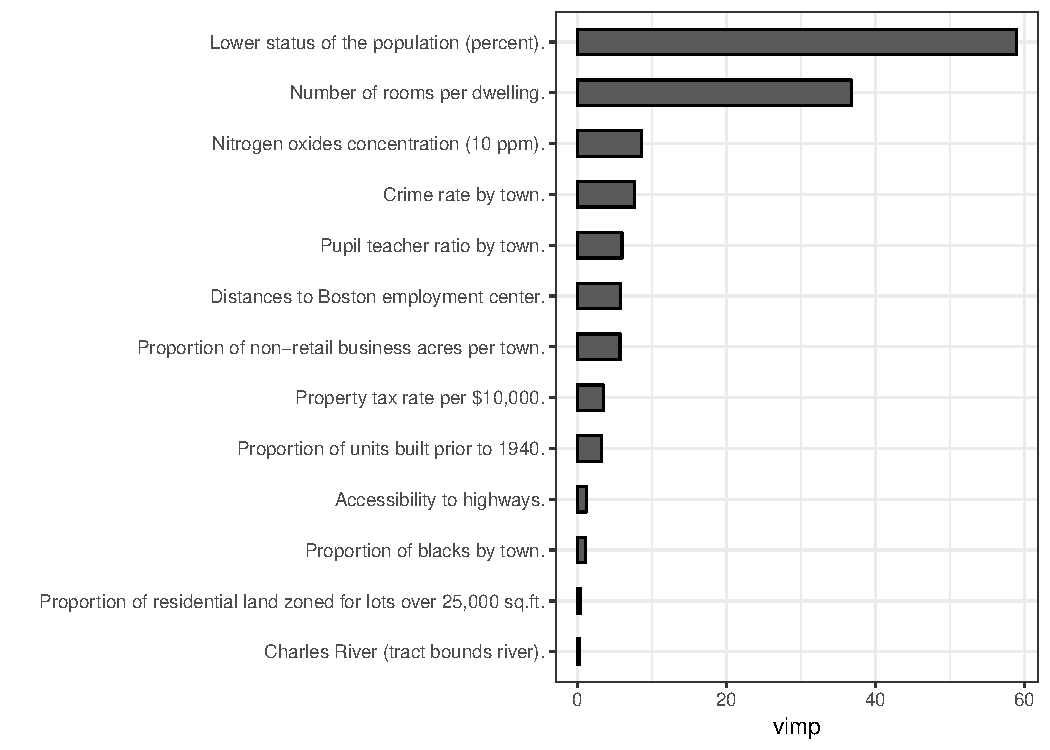
\includegraphics{Regression-rfsrc_files/figure-latex/vimp-1} 

}

\caption[Random forest VIMP plot]{Random forest VIMP plot. Bars are colored by sign of VIMP, longer blue bars indicate more important variables.}\label{fig:vimp}
\end{figure}
\end{CodeChunk}

For our random forest, the top two variables (\texttt{lstat} and
\texttt{rm}) have the largest VIMP, with a sizable difference to the
remaining variables, which mostly have similar VIMP measure. This
indicates we should focus attention on these two variables, at least,
over the others.

In this example, all VIMP measures are positive, though some are small.
When there are both negative and positive VIMP values, the
\texttt{plot.gg\_vimp} function will color VIMP by the sign of the
measure. We use the \texttt{lbls} argument to pass a named
\texttt{vector} of meaningful text descriptions to the
\texttt{plot.gg\_vimp} function, replacing the often terse variable
names used by default.

\subsection{Minimal Depth}\label{minimal-depth}

In VIMP, prognostic risk factors are determined by testing the forest
prediction under alternative data settings, ranking the most important
variables according to their impact on predictive ability of the forest.
An alternative method uses inspection of the forest construction to rank
variables. \emph{Minimal depth} assumes that variables with high impact
on the prediction are those that most frequently split nodes nearest to
the trunks of the trees (i.e.~at the root node) where they partition
large samples of the population.

Within a tree, node levels are numbered based on their relative distance
to the trunk of the tree (with the root at 0). Minimal depth measures
the important risk factors by averaging the depth of the first split for
each variable over all trees within the forest. Lower values of this
measure indicate variables important in splitting large groups of
patients.

The \emph{maximal subtree} for a variable \(x\) is the largest subtree
whose root node splits on \(x\). All parent nodes of \(x\)'s maximal
subtree have nodes that split on variables other than \(x\). The largest
maximal subtree possible is at the root node. If a variable does not
split the root node, it can have more than one maximal subtree, or a
maximal subtree may also not exist if there are no splits on the
variable. The minimal depth of a variables is a surrogate measure of
predictiveness of the variable. The smaller the minimal depth, the more
impact the variable has sorting observations, and therefore on the
forest prediction.

The \texttt{gg\_minimal\_depth} function is analogous to the
\texttt{gg\_vimp} function for minimal depth. Variables are ranked from
most important at the top (minimal depth measure), to least at the
bottom (maximal minimal depth). The vertical dashed line indicates the
minimal depth threshold where smaller minimal depth values indicate
higher importance and larger indicate lower importance.

The \texttt{randomForestSRC::var.select} call is again a computationally
intensive function, as it traverses the forest finding the maximal
subtree within each tree for each variable before averaging the results
we use in the \texttt{gg\_minimal\_depth} call. We again use the cached
object strategy here to save computational time. The \texttt{var.select}
call is included in the comment of this code block.

\begin{CodeChunk}

\begin{CodeInput}
R> # Load the data, from the call:
R> varsel_Boston <- var.select(rfsrc_Boston)
\end{CodeInput}

\begin{CodeOutput}
minimal depth variable selection ...


-----------------------------------------------------------
family             : regr 
var. selection     : Minimal Depth 
conservativeness   : medium 
x-weighting used?  : TRUE 
dimension          : 13 
sample size        : 506 
ntree              : 1000 
nsplit             : 0 
mtry               : 5 
nodesize           : 5 
refitted forest    : FALSE 
model size         : 11 
depth threshold    : 6.7242 
PE (true OOB)      : 10.8032 


Top variables:
        depth   vimp
lstat   1.135 58.948
rm      1.221 36.781
crim    2.516  7.685
nox     2.555  8.676
dis     2.573  5.834
ptratio 2.947  6.004
age     3.544  3.293
tax     3.644  3.497
black   3.767  1.135
indus   3.798  5.749
rad     6.117  1.251
-----------------------------------------------------------
\end{CodeOutput}

\begin{CodeInput}
R> # Save the gg_minimal_depth object for later use.
R> gg_md <- gg_minimal_depth(varsel_Boston)
R> 
R> # plot the object
R> plot(gg_md, lbls=st.labs)
\end{CodeInput}
\begin{figure}

{\centering 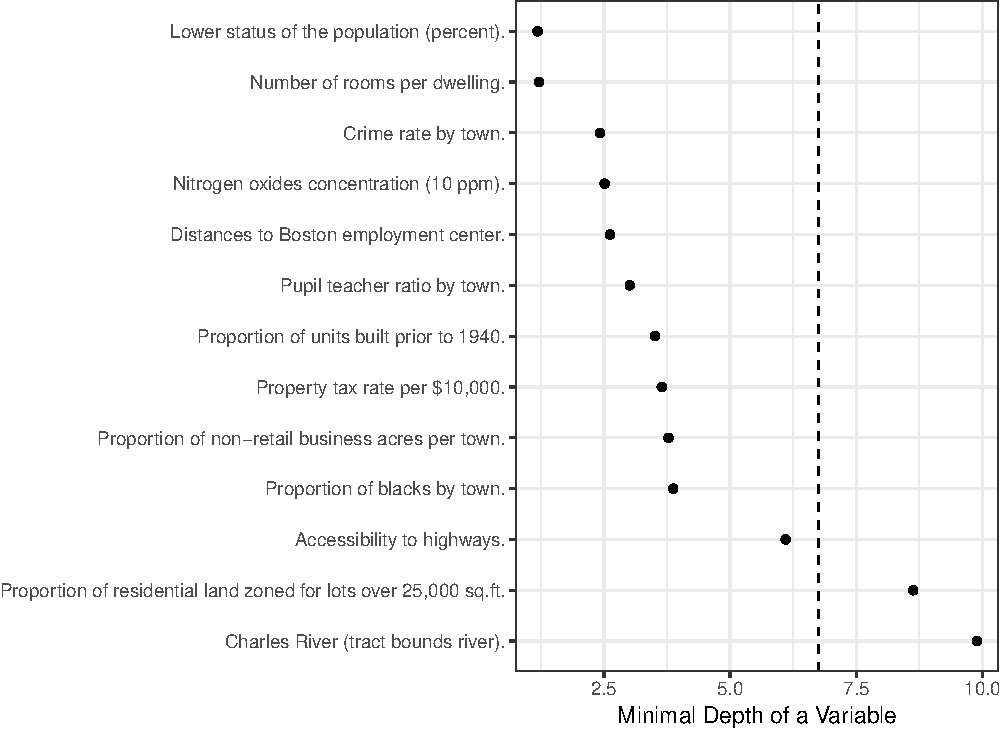
\includegraphics{Regression-rfsrc_files/figure-latex/minimaldepth-1} 

}

\caption[Minimal Depth variables in rank order, most important at the top]{Minimal Depth variables in rank order, most important at the top. Vertical dashed line indicates the maximal minimal depth for important variables.}\label{fig:minimaldepth}
\end{figure}
\end{CodeChunk}

In general, the selection of variables according to VIMP is to rather
arbitrarily examine the values, looking for some point along the ranking
where there is a large difference in VIMP measures. The minimal depth
threshold method has a more quantitative approach to determine a
selection threshold. Given minimal depth is a quantitative property of
the forest construction, \citep{Ishwaran:2010} also construct an
analytic threshold for evidence of variable impact. A simple optimistic
threshold rule uses the mean of the minimal depth distribution,
classifying variables with minimal depth lower than this threshold as
important in forest prediction. The minimal depth plot for our model
indicates there are ten variables which have a higher impact (minimal
depth below the mean value threshold) than the remaining three.

Since the VIMP and Minimal Depth measures use different criteria, we
expect the variable ranking to be somewhat different. We use
\texttt{gg\_minimal\_vimp} function to compare rankings between minimal
depth and VIMP. In this call, we plot the stored
\texttt{gg\_minimal\_depth} object (\texttt{gg\_md}), which would be
equivalent to calling \texttt{plot.gg\_minimal\_vimp(varsel\_Boston)} or
\texttt{plot(gg\_minimal\_vimp(varsel\_Boston))}.

\begin{CodeChunk}

\begin{CodeInput}
R> # gg_minimal_depth objects contain information about
R> # both minimal depth and VIMP.
R> plot(gg_minimal_vimp(gg_md))
\end{CodeInput}
\begin{figure}

{\centering 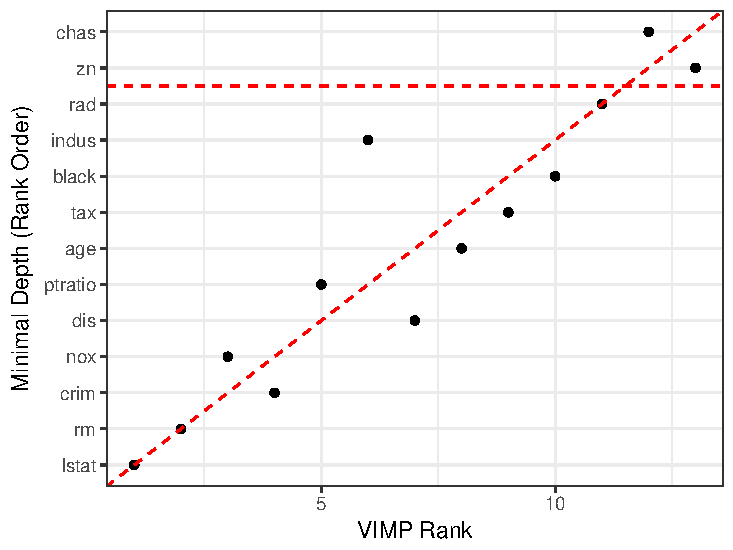
\includegraphics{Regression-rfsrc_files/figure-latex/minimalvimp-1} 

}

\caption[Comparing Minimal Depth and Vimp rankings]{Comparing Minimal Depth and Vimp rankings. Points on the red dashed line are ranked equivalently, points below have higher VIMP, those above have higher minimal depth ranking. Variables are colored by the sign of the VIMP measure.}\label{fig:minimalvimp}
\end{figure}
\end{CodeChunk}

The points along the red dashed line indicates where the measures are in
agreement. Points above the red dashed line are ranked higher by VIMP
than by minimal depth, indicating the variables are sensitive to
misspecification. Those below the line have a higher minimal depth
ranking, indicating they are better at dividing large portions of the
population. The further the points are from the line, the more the
discrepancy between measures. The construction of this figure is skewed
towards a minimal depth approach, by ranking variables along the y-axis,
though points are colored by the sign of VIMP.

In our example, both minimal depth and VIMP indicate the strong relation
of \texttt{lstat} and \texttt{rm} variables to the forest prediction,
which agrees with our expectation from the Data: Boston Housing Values
(\autoref{data-boston-housing-values}) done at the beginning of this
document. We now turn to investigating how these, and other variables,
are related to the predicted response.

\section{Response/Variable
Dependence}\label{responsevariable-dependence}

As random forests are not a parsimonious methodology, we can use the
minimal depth and VIMP measures to reduce the number of variables we
need to examine to a manageable subset. We would like to know how the
forest response depends on some specific variables of interest. We often
choose to examine variables of interest based on the study question, or
other previous knowledge. In the absence of this, we will look at
variables that contribute most to the predictive accuracy of the forest.

Although often characterized as a ``black box'' method, it is possible
to express a random forest in functional form. In the end the forest
predictor is some function, although complex, of the predictor variables
\[\hat{f}_{rf} = f(x).\] We use graphical methods to examine the forest
predicted response dependency on covariates. We again have two options,
Variable Dependence (\autoref{variable-dependence}) plots are quick and
easy to generate, and Partial Dependence
(\textbackslash{}autoref\{partial-dependence) plots are computationally
intensive but give us a risk adjusted look at the dependence.

\subsection{Variable Dependence}\label{variable-dependence}

Variable dependence plots show the predicted response as a function of a
covariate of interest, where each observation is represented by a point
on the plot. Each predicted point is an individual observations,
dependent on the full combination of all other covariates, not only on
the covariate of interest. Interpretation of variable dependence plots
can only be in general terms, as point predictions are a function of all
covariates in that particular observation. However, variable dependence
is straight forward to calculate, only requiring the predicted response
for each observation.

We use the \texttt{gg\_variable} function call to extract the training
set variables and the predicted OOB response from
\texttt{randomForestSRC::rfsrc} and \texttt{randomForestSRC::predict}
objects. In the following code block, we will store the
\texttt{gg\_variable} data object for later use, as all remaining
variable dependence plots can be constructed from this (\texttt{gg\_v})
object. We will also use the minimal depth selected variables (minimal
depth lower than the threshold value) from the previously stored
\texttt{gg\_minimal\_depth} object (\texttt{gg\_md\$topvars}) to filter
the variables of interest.

The \texttt{plot.gg\_variable} function call operates in the
\texttt{gg\_variable} object. We pass it the list of variables of
interest (\texttt{xvar}) and request a single panel
(\texttt{panel=TRUE}) to display the figures. By default, the
\texttt{plot.gg\_variable} function returns a list of \texttt{ggplot}
objects, one figure for each variable named in \texttt{xvar} argument.
The next three arguments are passed to internal \texttt{ggplot} plotting
routines. The \texttt{se} and \texttt{span} arguments are used to modify
the internal call to \texttt{ggplot2::geom\_smooth} for fitting smooth
lines to the data. The \texttt{alpha} argument lightens the coloring
points in the \texttt{ggplot2::geom\_point} call, making it easier to
see point over plotting. We also demonstrate modification of the plot
labels using the \texttt{ggplot2::labs} function.

\begin{CodeChunk}
\begin{figure}

{\centering 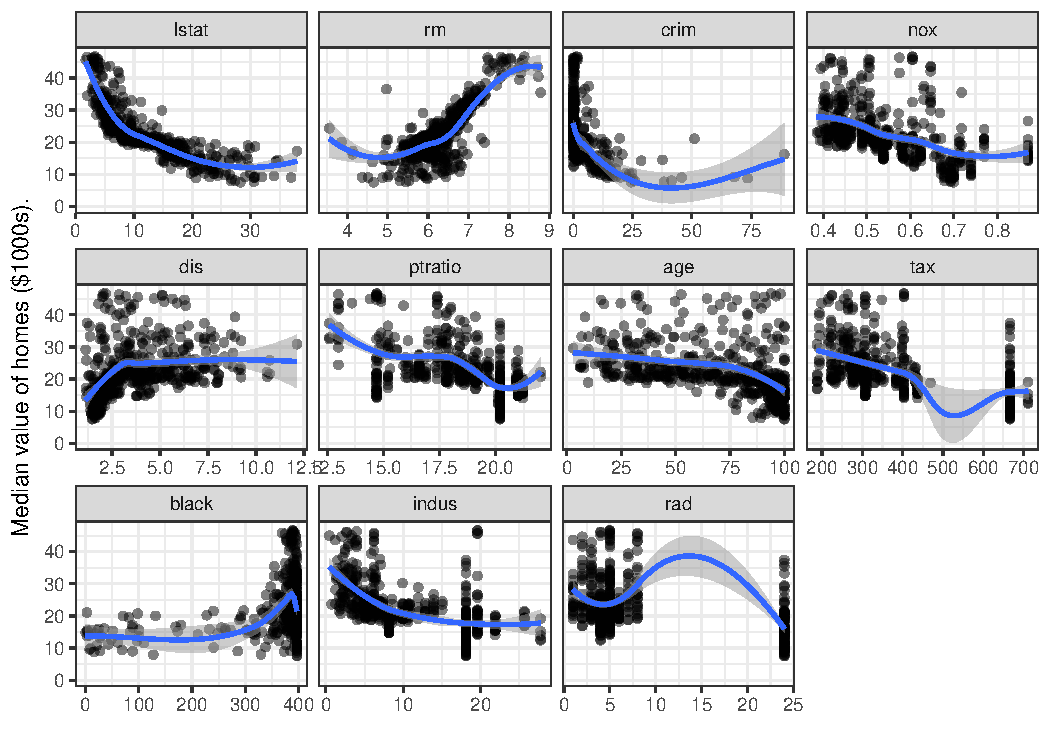
\includegraphics{Regression-rfsrc_files/figure-latex/variable-1} 

}

\caption[Variable dependence plot]{Variable dependence plot. Individual case predictions are marked with points. Loess smooth curve indicates the trend as the variables increase with shaded 95\% confidence band.}\label{fig:variable}
\end{figure}
\end{CodeChunk}

This figure looks very similar to the Data: Boston Housing Values
(\textbackslash{}autoref\{data-boston-housing-values) figure, although
with transposed axis as we plot the response variable on the y-axis. The
closer the panels match, the better the RF prediction. The panels are
sorted to match the order of variables in the \texttt{xvar} argument and
include a smooth loess line
\citep[\citet{cleveland:1988}]{cleveland:1981}, with 95\% shaded
confidence band, to indicates the trend of the prediction dependence
over the covariate values.

There is not a convenient method to panel scatter plots and boxplots
together, so we recommend creating panel plots for each variable type
separately. The Boston housing data does contain a single categorical
variable, the Charles river logical variable. Variable dependence plots
for categorical variables are constructed using boxplots to show the
distribution of the predictions within each category. Although the
Charles river variable has the lowest importance scores in both VIMP and
minimal depth measures, we include the variable dependence plot as an
example of categorical variable dependence.

\begin{CodeChunk}

\begin{CodeInput}
R> plot(gg_v, xvar="chas", alpha=.4)+
R+   labs(y=st.labs["medv"])
\end{CodeInput}
\begin{figure}

{\centering 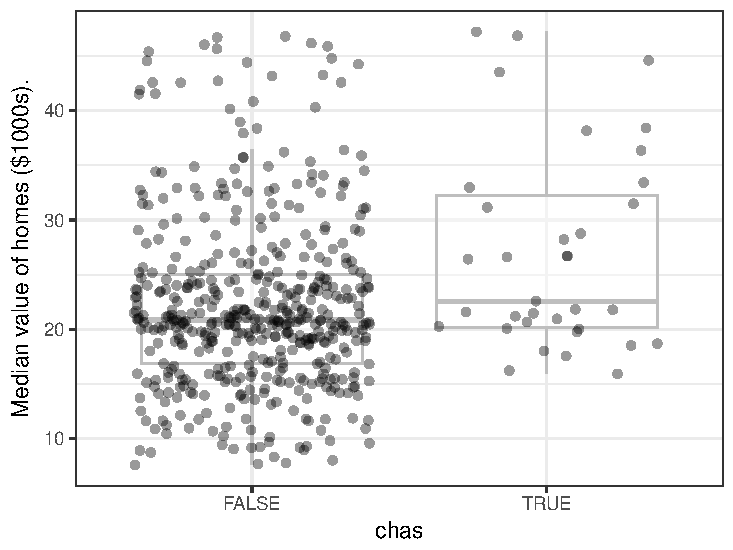
\includegraphics{Regression-rfsrc_files/figure-latex/chas-1} 

}

\caption[Variable dependence for Charles River logical variable]{Variable dependence for Charles River logical variable.}\label{fig:chas}
\end{figure}

\begin{CodeInput}
R> # , points=FALSE, se=FALSE, notch=TRUE
\end{CodeInput}
\end{CodeChunk}

The figure shows that most housing tracts do not border the Charles
river (\texttt{chas=FALSE}), and comparing the distributions of the
predicted median housing values indicates no significant difference in
home values. This reinforces the findings in both VIMP and Minimal
depth, the Charles river variable has very little impact on the forest
prediction of median home values.

\subsection{Partial Dependence}\label{partial-dependence}

Partial variable dependence plots are a risk adjusted alternative to
variable dependence. Partial plots are generated by integrating out the
effects of all variables beside the covariate of interest. Partial
dependence data are constructed by selecting points evenly spaced along
the distribution of the \(X\) variable of interest. For each value
(\(X = x\)), we calculate the average RF prediction over all other
covariates in \(X\) by
\[ \tilde{f}(x) = \frac{1}{n} \sum_{i = 1}^n \hat{f}(x, x_{i, o}), \]
where \(\hat{f}\) is the predicted response from the random forest and
\(x_{i, o}\) is the value for all other covariates other than \(X = x\)
for the observation \(i\) \citep{Friedman:2000}. Essentially, we average
a set of predictions for each observation in the training set at the
value of \(X=x\). We repeating the process for a sequence of \(X=x\)
values to generate the estimated points to create a partial dependence
plot.

Partial plots are another computationally intensive analysis, especially
when there are a large number of observations. We again turn to our data
caching strategy here. The default parameters for the
\texttt{randomForestSRC::plot.variable} function generate partial
dependence estimates at \texttt{npts=25} points (the default value)
along the variable of interest. For each point of interest, the
\texttt{plot.variable} function averages \texttt{n} response
predictions. This is repeated for each of the variables of interest and
the results are returned for later analysis.

\begin{CodeChunk}
\begin{figure}

{\centering 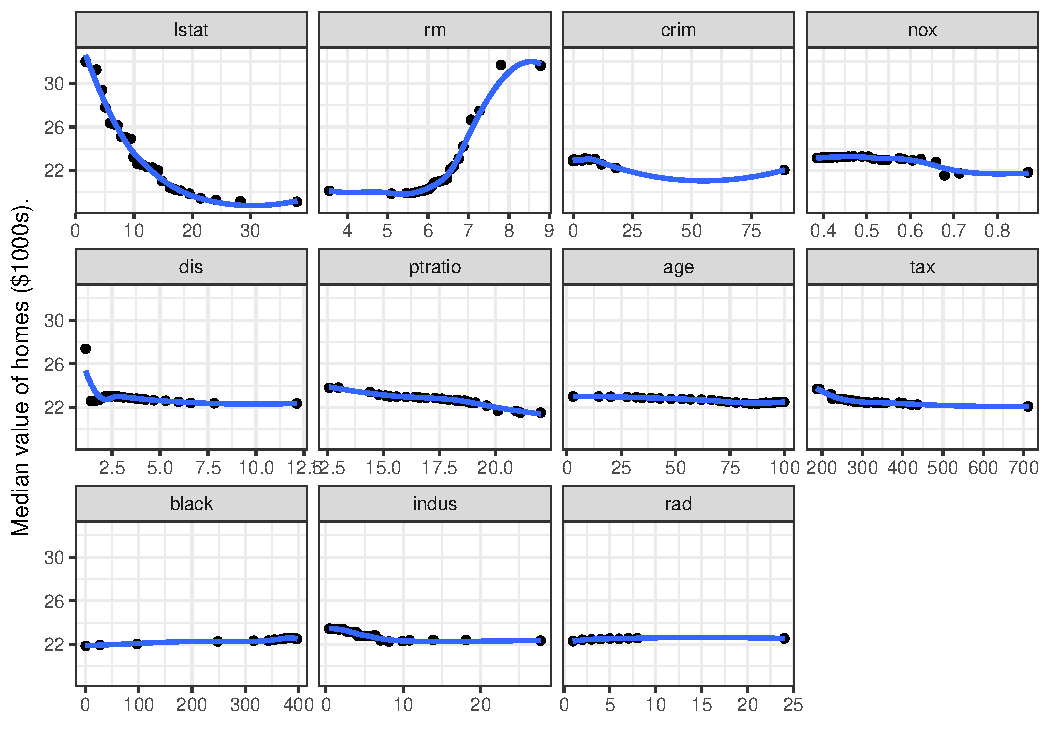
\includegraphics{Regression-rfsrc_files/figure-latex/partial-1} 

}

\caption[Partial dependence panels]{Partial dependence panels. Risk adjusted variable dependence for variables in minimal depth rank order.}\label{fig:partial}
\end{figure}
\end{CodeChunk}

We again order the panels by minimal depth ranking. We see again how the
\texttt{lstat} and \texttt{rm} variables are strongly related to the
median value response, making the partial dependence of the remaining
variables look flat. We also see strong nonlinearity of these two
variables. The \texttt{lstat} variable looks rather quadratic, while the
\texttt{rm} shape is more complex.

We could stop here, indicating that the RF analysis has found these ten
variables to be important in predicting the median home values. That
increasing \texttt{lstat} (percentage population of lower status) values
are associated with decreasing median home values (\texttt{medv}) and
increasing \texttt{rm\ \textgreater{}\ 6} (number of rooms \(> 6\)) are
associated with increasing median home values. However, we may also be
interested in investigating how these variables work together to help
improve the random forest prediction of median home values.

\section{Variable Interactions}\label{variable-interactions}

Using the different variable dependence measures, it is also possible to
calculate measures of pairwise interactions among variables. Recall that
minimal depth measure is defined by averaging the tree depth of variable
\(i\) relative to the root node. To detect interactions, this
calculation can be modified to measure the minimal depth of a variable
\(j\) with respect to the maximal subtree for variable \(i\)
\citep[\citet{Ishwaran:2011}]{Ishwaran:2010}.

The \texttt{randomForestSRC::find.interaction} function traverses the
forest, calculating all pairwise minimal depth interactions, and returns
a \(p \times p\) matrix of interaction measures. For each row, the
diagonal terms are are related to the minimal depth relative to the root
node, though normalized to minimize scaling issues. Each off diagonal
minimal depth term is relative to the diagonal term on that row. Small
values indicate that an off diagonal term typically splits close to the
diagonal term, indicating an forest split proximity of the two
variables.

The \texttt{gg\_interaction} function wraps the
\texttt{find.interaction} matrix for use with the provided plot and
print functions. The \texttt{xvar} argument indicates which variables
we're interested in looking at. We again use the cache strategy, and
collect the figures together using the \texttt{panel=TRUE} option.

\begin{CodeChunk}

\begin{CodeOutput}

                              Method: maxsubtree
                    No. of variables: 13
  Variables sorted by minimal depth?: TRUE

        lstat   rm crim  nox  dis ptratio  age black  tax indus  rad   zn chas
lstat    0.07 0.15 0.17 0.20 0.17    0.25 0.22  0.25 0.26  0.30 0.42 0.60 0.71
rm       0.15 0.08 0.21 0.23 0.19    0.26 0.23  0.25 0.26  0.31 0.41 0.59 0.73
crim     0.21 0.24 0.15 0.30 0.26    0.47 0.27  0.31 0.47  0.47 0.65 0.78 0.80
nox      0.24 0.28 0.28 0.17 0.29    0.49 0.34  0.36 0.50  0.54 0.66 0.78 0.83
dis      0.22 0.22 0.28 0.34 0.17    0.39 0.29  0.31 0.40  0.43 0.59 0.72 0.82
ptratio  0.28 0.26 0.37 0.43 0.34    0.20 0.34  0.38 0.43  0.47 0.60 0.73 0.84
age      0.27 0.27 0.32 0.42 0.31    0.47 0.23  0.34 0.46  0.46 0.63 0.78 0.83
black    0.34 0.35 0.40 0.52 0.39    0.58 0.38  0.25 0.59  0.58 0.70 0.86 0.88
tax      0.36 0.32 0.42 0.51 0.40    0.50 0.41  0.45 0.25  0.56 0.65 0.76 0.88
indus    0.39 0.37 0.45 0.55 0.45    0.55 0.43  0.47 0.54  0.25 0.70 0.79 0.86
rad      0.65 0.62 0.68 0.78 0.68    0.77 0.68  0.70 0.77  0.77 0.40 0.91 0.97
zn       0.83 0.79 0.86 0.89 0.85    0.89 0.83  0.86 0.89  0.89 0.94 0.56 0.98
chas     0.82 0.82 0.85 0.90 0.86    0.91 0.85  0.86 0.92  0.92 0.94 0.98 0.66
\end{CodeOutput}
\begin{figure}

{\centering 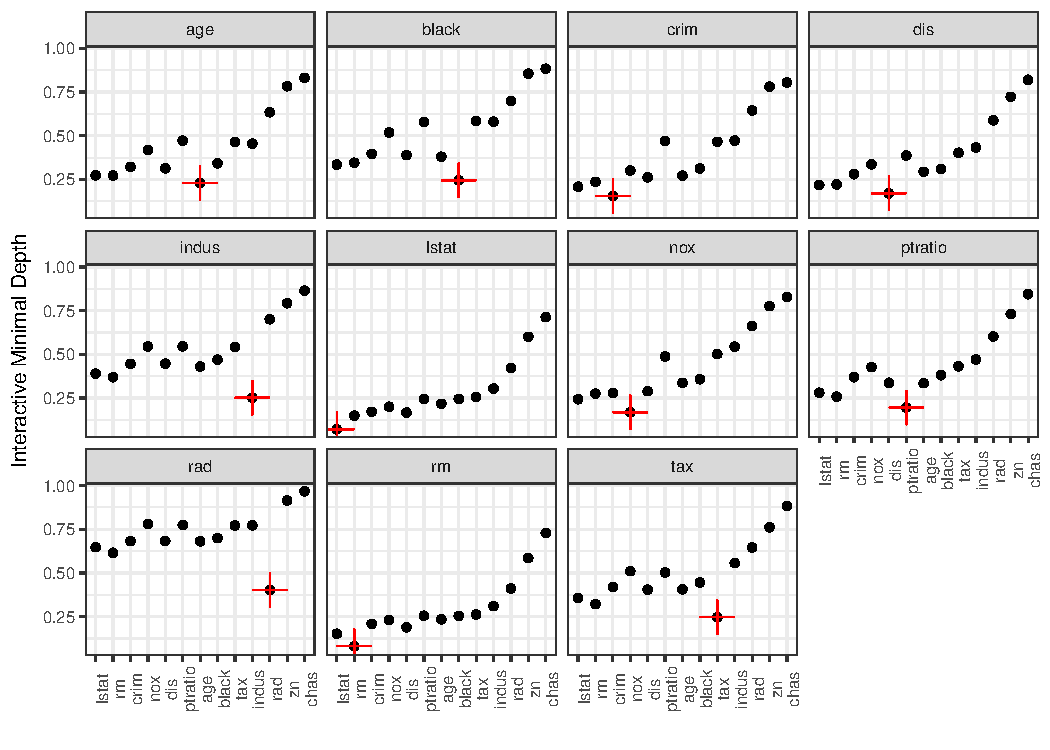
\includegraphics{Regression-rfsrc_files/figure-latex/interactions-1} 

}

\caption[Minimal depth variable interactions]{Minimal depth variable interactions. Reference variables are marked with red cross in each panel. Higher values indicate lower interactivity with reference variable.}\label{fig:interactions}
\end{figure}
\end{CodeChunk}

\autoref{fig:interactions} plots the interactions for the target
variable (shown in the red cross) with interaction scores for all
remaining variables. We expect the covariate with lowest minimal depth
(\texttt{lstat}) to be associated with almost all other variables, as it
typically splits close to the root node, so viewed alone it may not be
as informative as looking at a collection of interactive depth plots.
Scanning across the panels, we see each successive target depth
increasing, as expected. We also see the interactive variables
increasing with increasing target depth. Of interest here is the
interaction of \texttt{lstat} with the \texttt{rm} variable shown in the
\texttt{rm} panel. Aside from these being the strongest variables by
both measures, this interactive measure indicates the strongest
connection between variables.

\section{Coplots}\label{coplots}

Conditioning plots (coplots)
\citep[\citet{cleveland:1993}]{chambers:1992} are a powerful
visualization tool to efficiently study how a response depends on two or
more variables \citep{cleveland:1993}. The method allows us to view data
by grouping observations on some conditional membership. The simplest
example involves a categorical variable, where we plot our data
conditional on class membership, for instance on the Charles river
logical variable. We can view a coplot as a stratified variable
dependence plot, indicating trends in the RF prediction results within
panels of group membership.

Conditional membership with a continuous variable requires
stratification at some level. Often we can make these stratification
along some feature of the variable, for instance a variable with integer
values, or 5 or 10 year age group cohorts. However in the variables of
interest in our Boston housing example, we have no ``logical''
stratification indications. Therefore we will arbitrarily stratify our
variables into 6 groups of roughly equal population size using the
\texttt{quantile\_pts} function. We pass the break points located by
\texttt{quantile\_pts} to the \texttt{cut} function to create grouping
intervals, which we can then add to the \texttt{gg\_variable} object
before plotting with the \texttt{plot.gg\_variable} function. The simple
modification to convert variable dependence plots into condition
variable dependence plots is to use the \texttt{ggplot2::facet\_wrap}
command to generate a panel for each grouping interval.

We start by examining the predicted median home value as a function of
\texttt{lstat} conditional on membership within 6 groups of \texttt{rm}
``intervals''.

\begin{CodeChunk}
\begin{figure}

{\centering 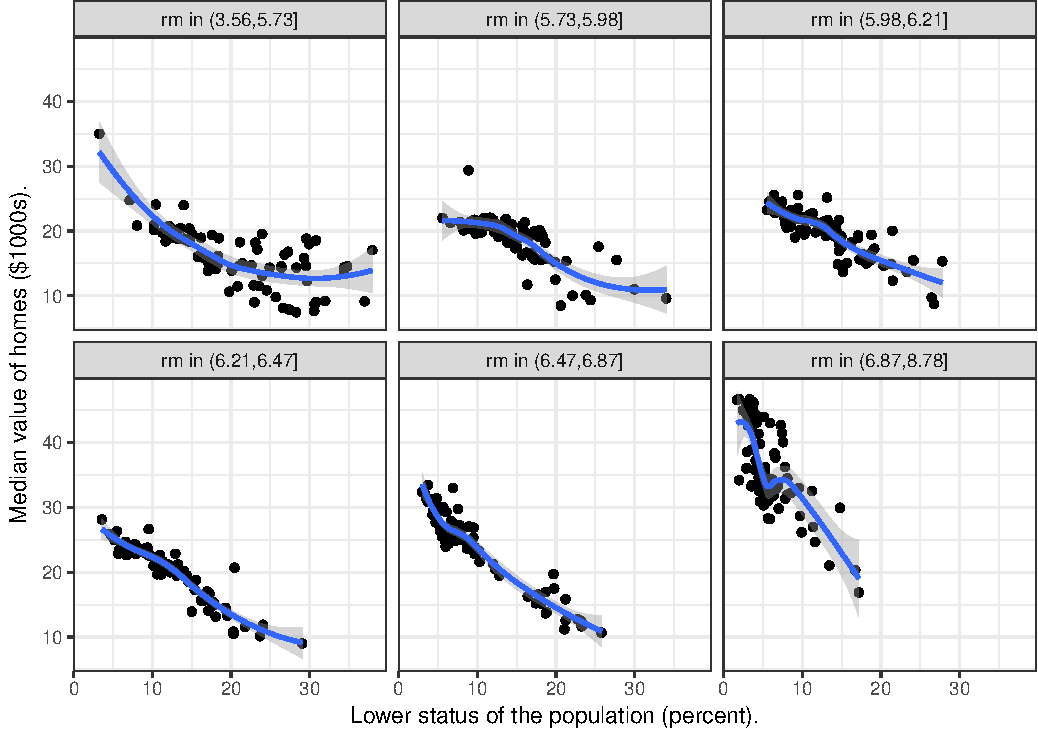
\includegraphics{Regression-rfsrc_files/figure-latex/coplots-1} 

}

\caption[Variable Coplots]{Variable Coplots. Predicted median home values as a function of percentage of lower status population, stratified by average number of rooms groups.}\label{fig:coplots}
\end{figure}
\end{CodeChunk}

Each point in this figure is the predicted median home value response
plotted against \texttt{lstat} value conditional on \texttt{rm} being on
the interval specified. We again use the smooth loess curve to get an
idea of the trend within each group. Overall, median values continue to
decrease with increasing \texttt{lstat}, and increases with increasing
\texttt{rm}. In addition to trends, we can also examine the conditional
distribution of variables. Note that smaller homes (\texttt{rm}) in high
status (lower \texttt{lstat}) neighborhoods still have high predicted
median values, and that there are more large homes in the higher status
neighborhoods (bottom right panel).

A single coplot gives us a grouped view of a variable (\texttt{rm}),
along the primary variable dimension (\texttt{lstat}). To get a better
feel for how the response depends on both variables, it is instructive
to look at the complement coplot. We repeat the previous coplot process,
predicted median home value as a function of the \texttt{rm} variable,
conditional on membership within 6 groups \texttt{lstat} intervals.

\begin{CodeChunk}
\begin{figure}

{\centering 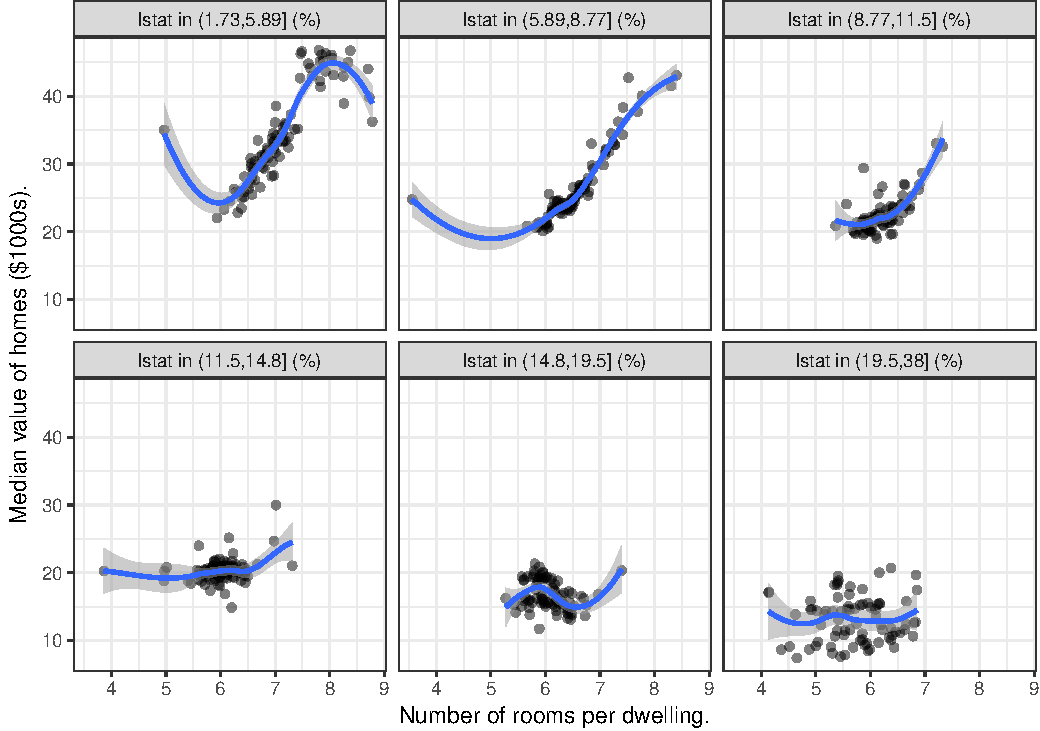
\includegraphics{Regression-rfsrc_files/figure-latex/coplots2-1} 

}

\caption[Variable Coplots]{Variable Coplots. Predicted median home value as a function of average number of rooms, stratified by percentage of lower status groups.}\label{fig:coplots2}
\end{figure}
\end{CodeChunk}

We get similar information from this view, predicted median home values
decrease with increasing \texttt{lstat} percentage and decreasing
\texttt{rm}. However viewed together we get a better sense of how the
\texttt{lstat} and \texttt{rm} variables work together (interact) in the
median value prediction.

Note that typically \citep{cleveland:1993} conditional plots for
continuous variables included overlapping intervals along the grouped
variable. We chose to use mutually exclusive continuous variable
intervals for multiple reasons:

\begin{itemize}
\item
  Simplicity - We can create the coplot figures directly from the
  \texttt{gg\_variable} object by adding a conditional group column
  directly to the object.
\item
  Interpretability - We find it easier to interpret and compare the
  panels if each observation is only in a single panel.
\item
  Clarity - We prefer using more space for the data portion of the
  figures than typically displayed in the \texttt{coplot} function
  available in base R, which require the bar plot to present the
  overlapping segments.
\end{itemize}

It is still possible to augment the \texttt{gg\_variable} to include
overlapping conditional membership with continuous variables by
duplicating rows of the object, and setting the correct conditional
group membership. The \texttt{plot.gg\_variable} function recipe above
could then be used to generate the panel plot, with panels ordered
according to the factor levels of the grouping variable. We leave this
as an exercise for the reader.

\subsection{Partial dependence
coplots}\label{partial-dependence-coplots}

By characterizing conditional plots as stratified variable dependence
plots, the next logical step would be to generate an analogous
conditional partial dependence plot. The process is similar to variable
dependence coplots, first determine conditional group membership, then
calculate the partial dependence estimates on each subgroup using the
\texttt{randomForestSRC::plot.variable} function with a the
\texttt{subset} argument for each grouped interval. The
\texttt{ggRandomForests::gg\_partial\_coplot} function is a wrapper for
generating a conditional partial dependence data object. Given a random
forest (\texttt{randomForestSRC::rfsrc} object) and a \texttt{groups}
vector for conditioning the training data set observations,
\texttt{gg\_partial\_coplot} calls the
\texttt{randomForestSRC::plot.variable} function for a set of training
set observations conditional on \texttt{groups} membership. The function
returns a \texttt{gg\_partial\_coplot} object, a sub class of the
\texttt{gg\_partial} object, which can be plotted with the
\texttt{plot.gg\_partial} function.

The following code block will generate the data object for creating
partial dependence coplot of the predicted median home value as a
function of \texttt{lstat} conditional on membership within the 6 groups
of \texttt{rm} ``intervals'' that we examined in the previous section.

\begin{CodeChunk}

\begin{CodeInput}
R> partial_coplot_Boston <- gg_partial_coplot(rfsrc_Boston, xvar="lstat", 
R+                                            groups=rm_grp,
R+                                            show.plots=FALSE)
\end{CodeInput}
\end{CodeChunk}

Since the \texttt{gg\_partial\_coplot} makes a call to
\texttt{randomForestSRC::plot.variable} for each group (6) in the
conditioning set, we again resort to the data caching strategy, and load
the stored result data from the \pkg{ggRandomForests} package. We modify
the legend label to indicate we're working with groups of the ``Room''
variable, and use the \texttt{palette="Set1"} from the
\texttt{RColorBrewer} package \citep{rcolorbrewer:2014} to choose a nice
color theme for displaying the six curves.

\begin{CodeChunk}

\begin{CodeInput}
R> # Load the stored partial coplot data.
R> 
R> # # Partial coplot
R> ggplot(partial_coplot_Boston, aes(x=lstat, y=yhat, col=group))+
R+   geom_point()+
R+   geom_smooth(se=FALSE, alpha=.25)+
R+   labs(x=st.labs["lstat"], y=st.labs["medv"],
R+        color="Room", shape="Room")+
R+   scale_color_brewer(palette="Set1")
\end{CodeInput}
\begin{figure}

{\centering 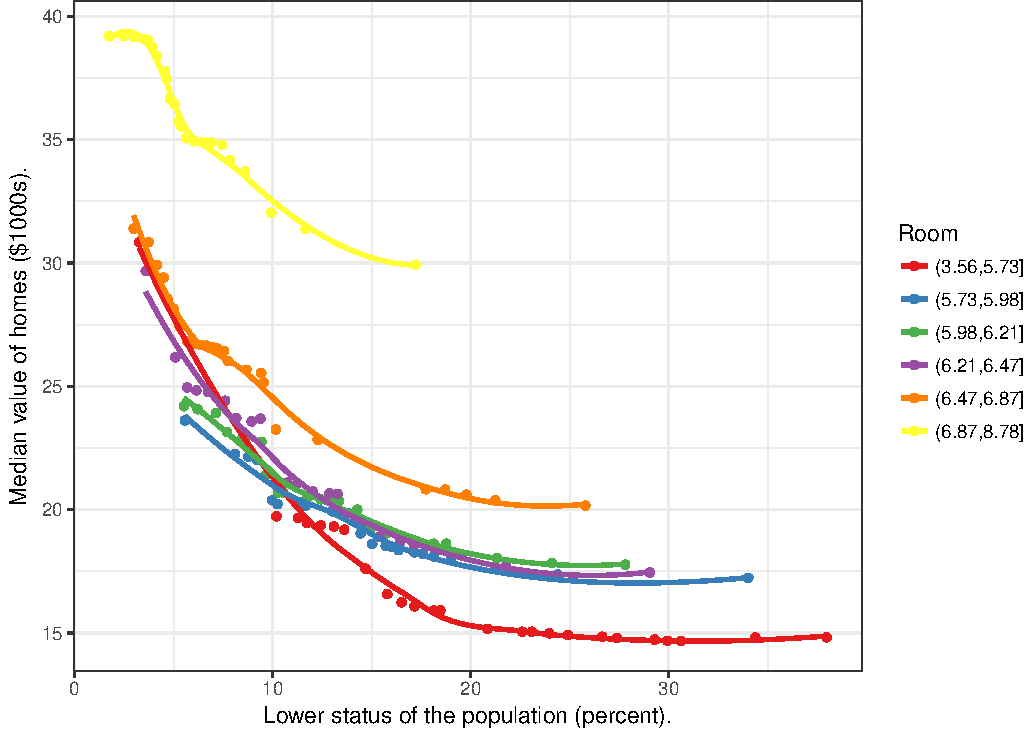
\includegraphics{Regression-rfsrc_files/figure-latex/prtl-coplots-1} 

}

\caption[Partial Coplots]{Partial Coplots. Risk adjusted predicted median value as a function of Lower Status, conditional on groups of average number of rooms.}\label{fig:prtl-coplots}
\end{figure}
\end{CodeChunk}

Unlike variable dependence coplots, we do not need to use a panel format
for partial dependence coplots because we are looking risk adjusted
estimates (points) instead of population estimates. The figure has a
loess curve through the point estimates conditional on the \texttt{rm}
interval groupings. The figure again indicates that larger homes
(\texttt{rm} from 6.87 and up, shown in yellow) have a higher median
value then the others. In neighborhoods with higher \texttt{lstat}
percentage, the Median values decrease with \texttt{rm} until it
stabilizes from the intervals between 5.73 and 6.47, then decreases
again for values smaller than 5.73. In lower \texttt{lstat}
neighborhoods, the effect of smaller \texttt{rm} is not as noticeable.

We can view the partial coplot curves as slices along a surface viewed
into the page, either along increasing or decreasing \texttt{rm} values.
This is made more difficult by our choice to select groups of similar
population size, as the curves are not evenly spaced along the
\texttt{rm} variable. We return to this problem in the next section.

We also construct the complement view, for partial dependence coplot of
the predicted median home value as a function of \texttt{rm} conditional
on membership within the 6 groups of \texttt{lstat} ``intervals'', and
cache the following \texttt{gg\_partial\_coplot} data call, and plot the
results with the \texttt{plot.gg\_variable} call:

\begin{CodeChunk}

\begin{CodeInput}
R> partial_coplot_Boston2 <- gg_partial_coplot(rfsrc_Boston, xvar="rm", 
R+                                             groups=lstat_grp,
R+                                             show.plots=FALSE)
\end{CodeInput}
\end{CodeChunk}

\begin{CodeChunk}

\begin{CodeInput}
R> # Partial coplot
R> #plot(partial_coplot_Boston2)+ ## again plot.gg_partial_coplot
R> ggplot(partial_coplot_Boston2, aes(x=rm, y=yhat, col=group))+
R+   geom_point()+
R+   geom_smooth(se=FALSE)+
R+   labs(x=st.labs["rm"], y=st.labs["medv"], 
R+        color="Lower Status", shape="Lower Status")+
R+   scale_color_brewer(palette="Set1")
\end{CodeInput}
\begin{figure}

{\centering 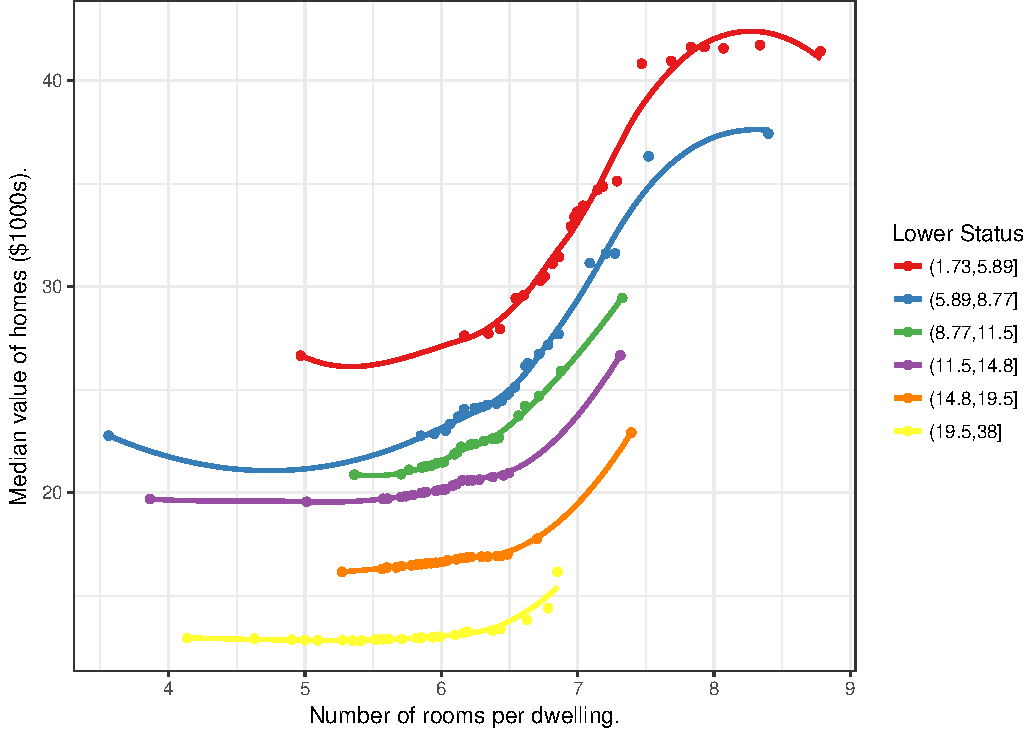
\includegraphics{Regression-rfsrc_files/figure-latex/prtl-coplots2-1} 

}

\caption[Partial Coplots]{Partial Coplots. Risk adjusted predicted median value as a function of average number of rooms, conditional on groups of percentage of lower status population.}\label{fig:prtl-coplots2}
\end{figure}
\end{CodeChunk}

This figure indicates that the median home value does not change much
until the \texttt{rm} increases above 6.5, then flattens again above 8,
regardless of the \texttt{lstat} value. This agrees well with the
\texttt{rm} Partial Dependence
(\textbackslash{}autoref\{partial-dependence) plots shown earlier.
Again, care must be taken in interpreting the even spacing of these
curves along the percentage of \texttt{lstat} groupings, as again, we
chose these groups to have similar sized populations, not to be evenly
spaced along the \texttt{lstat} variable.

\section{Partial plot surfaces}\label{partial-plot-surfaces}

Visualizing two dimensional projections of three dimensional data is
difficult, though there are tools available to make the data more
understandable. To make the interplay of lower status and average room
size a bit more understandable, we will generate a contour partial plot
of the median home values. We could generate this figure with the coplot
data we already have, but the resolution would be a bit strange. To
generate the plot of \texttt{lstat} conditional on \texttt{rm}
groupings, we would end up with contours over a grid of \texttt{lstat}=
\(25 \times\) \texttt{rm}= \(6\), for the alternative \texttt{rm}
conditional on \texttt{lstat} groups, we'd have the transpose grid of
\texttt{lstat}= \(6 \times\) \texttt{rm}= \(25\).

Since we are already using the data caching strategy, we will generate
another set of \texttt{gg\_partial} objects with increased resolution in
both the \texttt{lstat} and \texttt{rm} dimensions. For this exercise,
we will find 50 points evenly spaced along the \texttt{rm} variable
values, and generate a partial plot curve for each point. For these
partial plots, we will evaluate the risk adjusted median home value over
\texttt{npts=50} points along the \texttt{lstat} variable. This code
block finds 50 \texttt{rm} values evenly spaced along the distribution
of \texttt{rm}.

\begin{CodeChunk}

\begin{CodeInput}
R> # Find the quantile points to create 50 cut points
R> rm_pts <- quantile_pts(rfsrc_Boston$xvar$rm, groups=49, intervals = TRUE)
\end{CodeInput}
\end{CodeChunk}

We use the following data call to generate the partial plots with the
\texttt{randomForestSRC::plot.variable} call. Within the lapply call, we
use scope to modify the value of the \texttt{rm} variable within the
\texttt{rfsrc\_Boston} training set. Since all values in the training
set are the same, the averaged value of \texttt{rm} places each partial
plot curve at a specific value of \texttt{rm}. This code block took
about 20 minutes to run on a quad core Mac Air using a single processor.

The cached data is stored in the \texttt{partial\_Boston\_surf} data set
in the \pkg{ggRandomForests} package. The data set is a \texttt{list} of
50 \texttt{plot.variable} objects. This code block loads the data,
converts the \texttt{plot.variable} objects to \texttt{gg\_partial}
objects, attaches numeric values for the \texttt{rm} variable, and
generates the contour plot.

\begin{CodeChunk}

\begin{CodeInput}
R> # Generate the gg_partial_coplot data object
R> system.time(partial_Boston_surf <- lapply(rm_pts, function(ct){
R+   rfsrc_Boston$xvar$rm <- ct
R+   plot.variable(rfsrc_Boston, xvar = "lstat", time = 1,
R+                 npts = 50, show.plots = FALSE, 
R+                 partial = TRUE)
R+ }))
\end{CodeInput}

\begin{CodeOutput}
   user  system elapsed 
  93.16    0.00   93.19 
\end{CodeOutput}

\begin{CodeInput}
R> #     user   system  elapsed 
R> # 1109.641   76.516 1199.732 
\end{CodeInput}
\end{CodeChunk}

\begin{CodeChunk}
\begin{figure}

{\centering 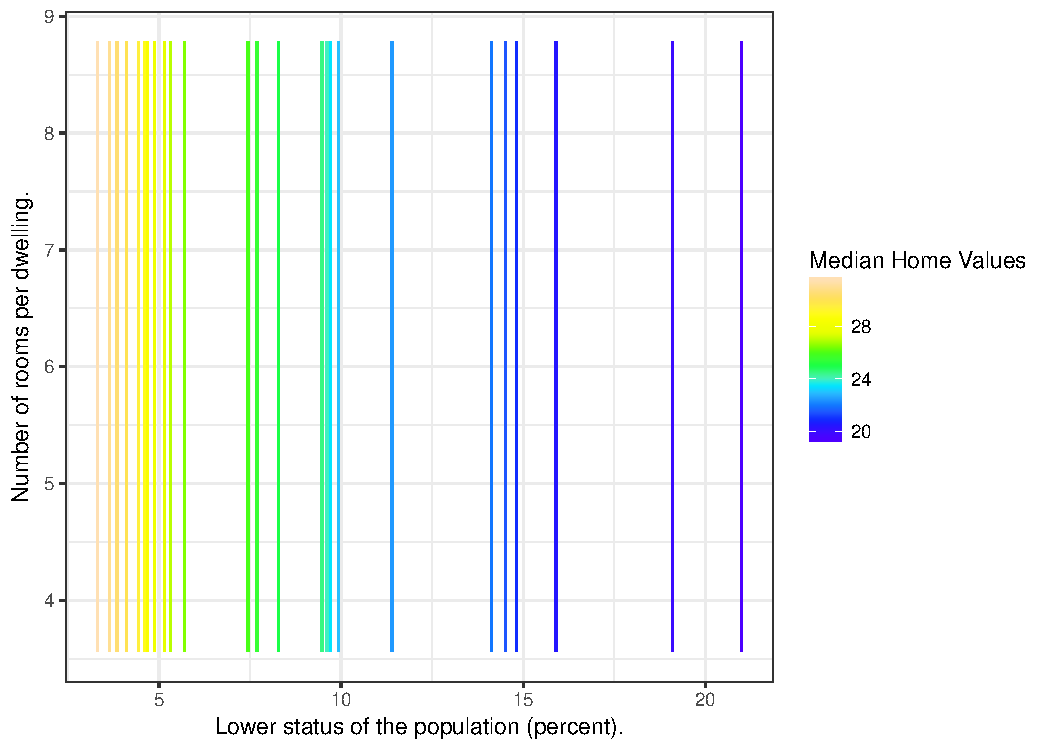
\includegraphics{Regression-rfsrc_files/figure-latex/contour3d-1} 

}

\caption[Partial coplot contour plot]{Partial coplot contour plot. Contours of median home value along the lstat/rm plane.}\label{fig:contour3d}
\end{figure}
\end{CodeChunk}

The contours are generated over the raw \texttt{gg\_partial} estimation
points, not smooth curves as shown in the Partial Dependence
(\textbackslash{}autoref\{partial-dependence) plots and Partial Coplots
(\textbackslash{}autoref\{partial-dependence-coplots) figures
previously. Contour lines, like topographic maps, are concentrated where
the slope of the surface is large. We use color to indicate the
direction of the contour lines, so that lower median home values are
concentrated in the lower right hand corner, and the values increase
along the diagonal toward the upper right. The close contour lines
indicate some thing like a step in values at 7 and 7.5 rooms, and at 5,
10 and 15\% lstat.

Contour plots are still a little difficult to interpret. However, we can
also generate a surface with this data using the \pkg{plot3D} package
\citep{plot3D:2014} and the \texttt{plot3D::surf3D} function. Viewed in
3D, a surface can help to better understand what the contour lines are
showing us.

\begin{CodeChunk}
\begin{figure}

{\centering 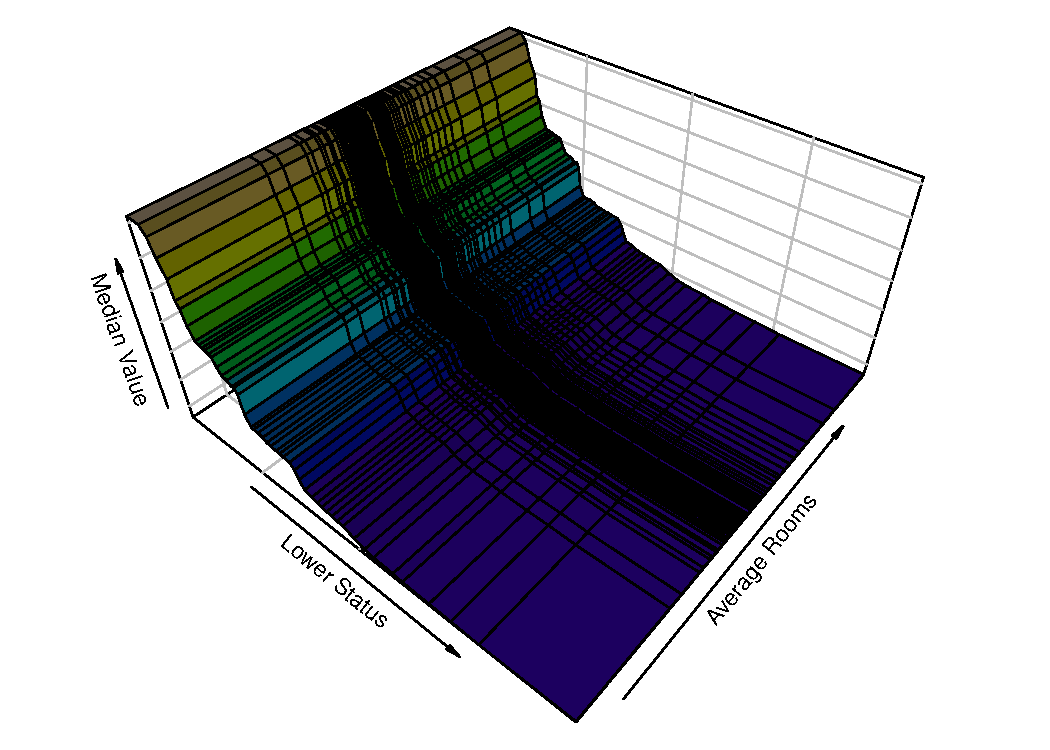
\includegraphics{Regression-rfsrc_files/figure-latex/surface3d-1} 

}

\caption[Partial plot surface]{Partial plot surface.}\label{fig:surface3d}
\end{figure}
\end{CodeChunk}

These figures reinforce the previous findings, where lower home values
are associated with higher \texttt{lstat} percentage, and higher values
are associated with larger \texttt{rm}. The difference in this figure is
we can see how the predicted values change as we move around the map of
\texttt{lstat} and \texttt{rm} combinations. We do still need to be
careful though, as partial plots average over values on the surface that
are note supported by actual observations.

\section{Conclusion}\label{conclusion}

In this vignette, we have demonstrated the use of the
\pkg{ggRandomForests} package to explore a regression random forest
built with the \pkg{randomForestSRC} package. We have shown how to
create a random forest (\autoref{random-forest---regression}) model and
determine which variables contribute to the forest prediction accuracy
using both VIMP (\autoref{variable-importance}) and Minimal Depth
(\autoref{minimal-depth}) measures. We outlined how to investigate
variable associations with the response variable using variable
dependence (\autoref{variable-dependence}) and the risk adjusted partial
dependence (\autoref{partial-dependence}) plots. We've also explored
variable interactions by using pairwise minimal depth interactions
(\autoref{variable-interactions}) and directly viewed these interactions
using variable dependence coplots (\autoref{coplots}) and partial
dependence coplots (\autoref{partial-dependence-coplots}). Along the
way, we've demonstrated the use of additional commands from the
\pkg{ggplot2} package for modifying and customizing results from
\pkg{ggRandomForests}.

\renewcommand\refname{References}
\bibliography{ggRandomForestsRMD}


\end{document}

